\section{Verwendung}
\fib{}
\subsection{Hilfe}
\noindent
Um die Hilfe aufzurufen kann man einen der beiden folgenden Befehle verwenden:
\begin{itemize}
    \item ``ermtk --help,,
    \item ``ermtk -h,,
\end{itemize}

\begin{figure}[H]
	\begin{center}
		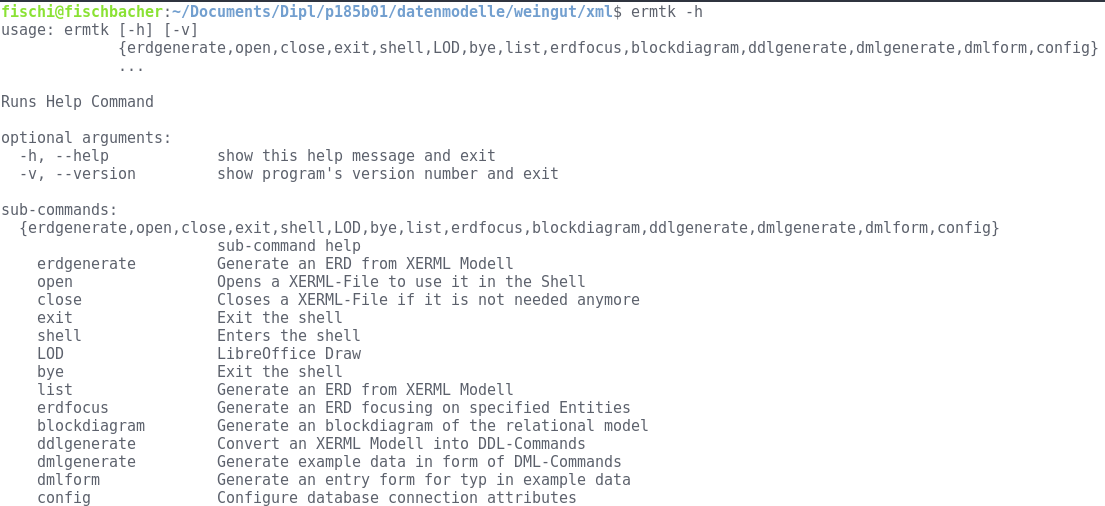
\includegraphics[width=16cm, height=10cm]{images/ermtk_help.png}
		\caption{Ausgabe vom help Befehl}
		\label{dot}
	\end{center}
\end{figure}

\subsection{Programm Aufruf}
\fib{}
Das die ERMTK-Repl Shell gestartet wird muss man den Befehl ``ermtk shell,, eingeben. Man merkt das man sich in der ERMTK-Repl Shell befindet, an dem Prompt ``ermtk>,,.

\begin{figure}[H]
	\begin{center}
		
\includegraphics[width=17 cm, height=1cm]{images/ermtk_shell.png}
		\caption{Aufruf der ERMTK-Repl Shell und öffnen einer Datei}
		\label{open}
	\end{center}
\end{figure}

\noindent
Um dann eine Datei zu öffnen muss man den Befehl ``open <inputfile>,,, wie in Abbildung 6.2 dargestellt, verwenden.

\subsection{``erdgenerate,,}

\begin{figure}[H]
	\begin{center}
		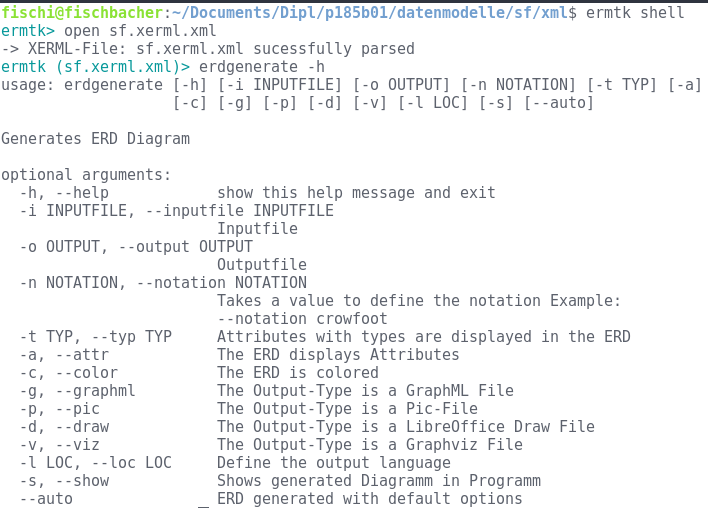
\includegraphics[width=16cm, height=10cm]{images/help.png}
		\caption{Ausgabe der hilfe zum Befehl erdgenerate}
		\label{erdgenerate}
	\end{center}
\end{figure}

\noindent
Nachdem man eine Datei geöffnet hat kann man mittels ``erdgenerate,, sich ein Entity-Relationship Diagramm generieren lassen, dabei hat man die Auswahl zwischen vier verschiedenen Varianten:
\begin{itemize}
    \item -g, --graphml um den Graphen mittels Graphml zu generieren.
    \item -p, --pic um den Graphen mittels PIC-Code zu generieren.
    \item -d, --draw um den Graphen mittels LibreOffice Draw zu generieren.
    \item -v, --viz um den Graphen mittels Graphviz zu generieren.
\end{itemize}
\fib{}
\noindent
Außerdem hat man die Möglichkeit mit dem Parameter ``-c,, oder ``--color,, sich den den Graphen farbig zu generieren lassen und mit dem Parameter ``-a,, oder ``--attr,, ob man Attribute auch generiert haben will.
Die ERMTK-Repl Shell kann man jederzeit mit den Befehlen ``exit,, oder ``close,, verlassen.